\documentclass[12pt]{article}
\usepackage[utf8]{inputenc}
\usepackage[T1]{fontenc}
\usepackage{fontspec}
\setmainfont{Times New Roman}
\newfontfamily\hackfont{Hack}
\usepackage{titlesec}
\usepackage{fancyhdr}
\usepackage{listings}
\usepackage{xcolor}
\usepackage{graphicx}
\usepackage{longtable}
\usepackage{caption}
\usepackage{hyperref}
\usepackage{setspace}
\usepackage{geometry}
\geometry{a4paper, margin=1in}
\hypersetup{colorlinks=true, linkcolor=blue, urlcolor=blue}
\renewcommand{\contentsname}{Table of Contents}

\pagestyle{fancy}
\fancyhf{} 							% Header Middle
\rhead{VLSI Design Lab}
\lhead{Lab-04: FlipFlop Circuit}
\rfoot{\thepage}

\begin{document}

\begin{titlepage}					% Cover Start
\begin{center}
    
\includegraphics[width=0.35\textwidth]{logo.png} \\
    \vspace{0.5cm}
    \textbf{\Huge \textcolor{cyan}{NOTRE DAME} \textcolor{cyan}{UNIVERSITY}} \\
    \vspace{0.5cm}
    \textbf{\Huge \textcolor{orange}{BANGLADESH}} \\
    
    \vspace{0.9cm}
    \textbf{\Huge \underline{VLSI Design Lab Report-04}} \\
    
    \vspace{1.5em}
    \begin{flushleft}
    	\textbf{\Large Course Code: CSE-4218} \\
		\vspace{0.3cm}        
        \textbf{\Large Course Title: VLSI Design Lab} \\
        \vspace{0.3cm}
        \textbf{\Large Experiment Name: Implementing FlioFlop Circuit} \\        
    \end{flushleft}
    
    \vspace{1em}
    \begin{flushleft}
        \textbf{\Huge \textcolor{blue}{Submitted by:}} \\
        \vspace{0.3cm}
        \textbf{\Large Name: Istiak Alam} \\
        \vspace{0.3cm}
        \textbf{\Large ID: 0692230005101005} \\
		\vspace{0.3cm}        
        \textbf{\Large Batch: CSE-20} \\
        \vspace{0.5cm}
        \textbf{\Large Submission Date: }{\Large \textbf{\today}\par}
    \end{flushleft}
    \vfill
    \begin{flushleft}
        \textbf{\Huge \textcolor{blue}{Submitted to:}} \\
        \vspace{0.3cm}
        \textbf{\Large Nafisa Tabassum,} \\
        \vspace{0.3cm}
        \textbf{\Large Lecturer, Dept. of CSE} \\
        \vspace{0.3cm}
        \textbf{\Large Notre Dame University Bangladesh}
    \end{flushleft}
\end{center}
\end{titlepage}						% Cover End

\tableofcontents
\thispagestyle{empty}
\clearpage
\pagenumbering{arabic}

\section*{\center Abstract}
This laboratory experiment presents the design and CMOS implementation of a flip-flop circuit using the DSCH2 schematic simulation tool. A D Flip-Flop was realized using CMOS logic principles and its functional behavior was verified through truth table analysis and timing simulation. The circuit operation was analyzed with respect to clock-triggered input transitions, and the timing diagram was used to observe the synchronization between input and output signals. The experimental results confirm that the implemented flip-flop exhibits correct edge-triggered behavior and maintains stable data storage, consistent with theoretical expectations.


\section{Introduction}
This laboratory experiment focuses on the design and implementation of a flip-flop circuit using CMOS logic in the DSCH2 environment. Flip-flops are fundamental sequential elements used for data storage and synchronization in digital systems. In this experiment, a D Flip-Flop was designed using CMOS-based logic gates, and its functionality was verified through truth table analysis and timing simulation. The behavior of the circuit was observed with respect to clock-triggered input transitions.

\section{Objective}
The objectives of this laboratory experiment are as follows:
\begin{itemize}
    \item To design and implement a flip-flop circuit using CMOS logic.
    \item To develop schematic-level circuits using the DSCH2 tool.
    \item To derive and verify the truth table of the flip-flop from simulation.
    \item To analyze timing diagrams to observe clock-triggered behavior.
    \item To understand the operation of sequential circuits and data storage elements.
\end{itemize}

\section{Function}
The D Flip-Flop is a clock-controlled bistable device that transfers the input data (D) to the output (Q) on the active edge of the clock signal.

\[
Q_{next} = D
\]

The output changes only at the triggering edge of the clock, ensuring synchronized data storage.


\subsection*{Truth Table}
\begin{center}
\begin{tabular}{|c|c|c|}
\hline
Clock & D & Q(next) \\ \hline
$\uparrow$ & 0 & 0 \\
$\uparrow$ & 1 & 1 \\
No Edge & X & Q(previous) \\ \hline
\end{tabular}
\end{center}

\subsection*{Schematic Image}
\begin{figure}[!h]
\centering
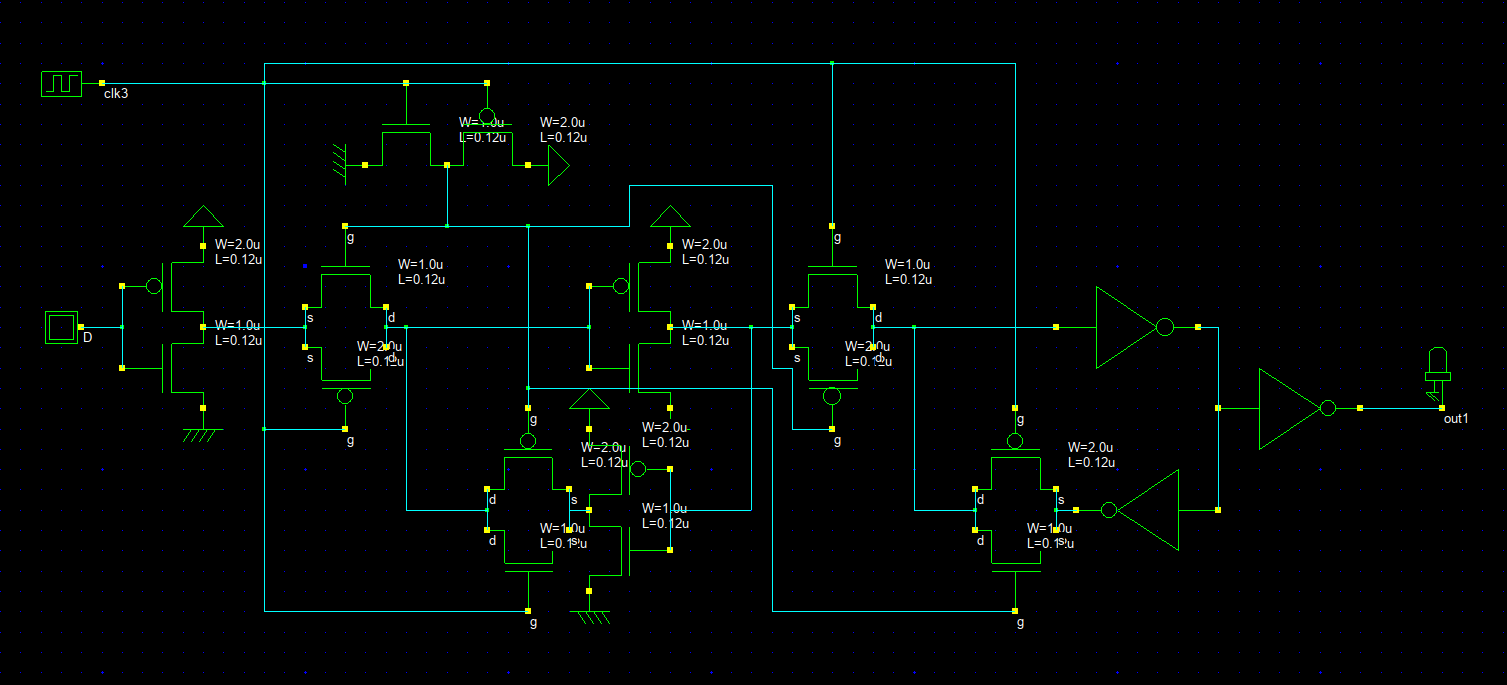
\includegraphics[width=1\textwidth]{FlipFlop.png}
\caption{CMOS Schematic of D Flip-Flop in DSCH2}
\end{figure}


\subsection*{Timing Diagram}
\begin{figure}[!h]
\centering
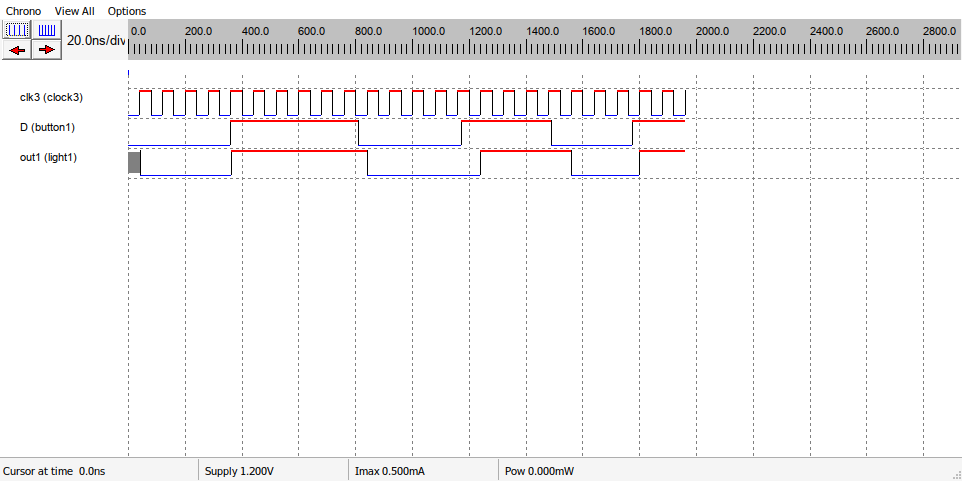
\includegraphics[width=1\textwidth]{Timing Diagram.png}
\caption{Timing Diagram of D Flip-Flop}
\end{figure}

The timing diagram shows that the output Q follows the input D only at the rising edge of the clock signal. Between clock edges, the output remains constant regardless of changes in the input. \\
From the simulation results, it was observed that the D Flip-Flop changes its output state only at the rising edge of the clock signal. When the clock transitions from LOW to HIGH, the output Q takes the value of the input D. At all other times, the output remains unchanged, preserving the previously stored value. This behavior confirms the correct operation of the edge-triggered D Flip-Flop implemented using CMOS logic.

% =====================================================
\section{Conclusion}
The CMOS-based D Flip-Flop was successfully designed and simulated using the DSCH2 tool. The truth table and timing diagram verified that the circuit operates correctly as a clocked storage element. This experiment reinforces the understanding of sequential logic design and the role of flip-flops in digital systems.


\end{document}